The AUC and prediction rate of predicting future cyber attacks using PLP on the data set described in \secref{cyberattacks} is shown in \figref{fig:plp_auc} for different lengths of the set used for testing. We find that the AUC increases around 10 percent units from 1 month of prediction data to 24 months of prediction data. However, the prediction rate does not vary that much for length of prediction data of at least 6 months.

\begin{figure}[!ht]
\centering
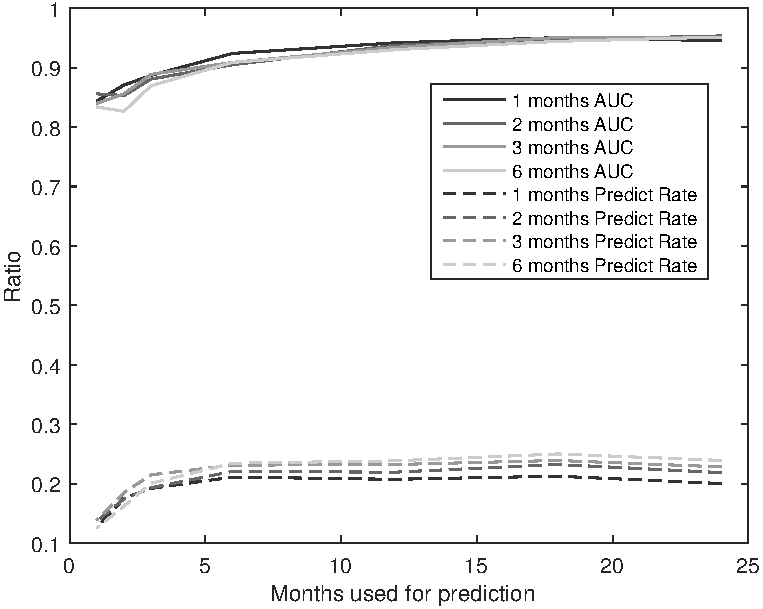
\includegraphics[scale=0.9]{images/auc_plp_result.pdf}
\caption{\label{fig:plp_auc} AUC and prediction rate for the PLP algorithm used on the cyber attack bipartite graph. The different shades of grays represent differents length of time period used for testing (in months). AUC was calculated according to the description in section \ref{plp:auc} and prediction rate according to \ref{plp:predict_rate}.}
\end{figure}

An example output of predicted attacks is shown in table \ref{tab:example_attacks}. Only the 10 predicted attacks with highest prediction values is shown. Notice how some attacks seems unlikely, for example that Election Commission of India would cyberattack moneycontrol.com. This is because methods of extracting information is not perfect since it is based on natural language processing algorithms. 

\begin{table}[]
    \centering
    \begin{tabular}{|l|l|c|}\hline
 Attacker & Target & Prediction Value \\  \hline
 Monte Melkonian Cyber Army & Banking & 0.33 \\
 Organization of Petroleum Exporting Countries & Petróleos Mexicanos & 0.33 \\
 Election Commission of India & moneycontrol.com & 0.33 \\
 Indonesian Security Down & Tok & 0.33 \\
 United Kingdom & United States & 0.32 \\
 PT28 Fancy Bear & Twitter & 0.29 \\
 Anonymous Scandinavia & United States & 0.26 \\
 Russian hackers & Microsoft & 0.24 \\ 
 Shadow Brokers & Twitter & 0.24 \\
 Russian hackers & Iran & 0.24 \\ \hline
    \end{tabular}
    \caption{Predicted attacks using 6 months of prediction data, showing only the 10 out of 1 million predicted attacks with the highest prediction values.}
    \label{tab:example_attacks}
\end{table}

How great the natural limitations of the algorithm are can be seen in \figref{fig:plp_max} where the maximum possible prediction rate, the ratio of cyber attacks with same actors as was previously seen in the prediction set and the ratio of cyber attacks that involved at least one new actor is presented.

\begin{figure}[!ht]
\centering
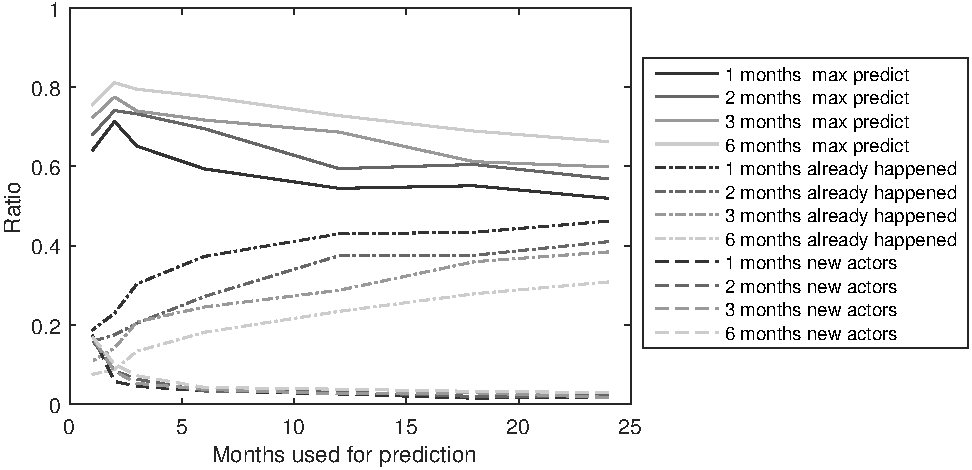
\includegraphics[width=\textwidth]{images/max_plp_result.pdf}
\caption{\label{fig:plp_max} 
Maximum prediction rate possible for PLP for comparison with the prediction rate in \figref{fig:plp_auc}. Also showing the ratio of attacks with set of actors already in prediction set as well as the ratio of attacks involving at least one new actor.}
\end{figure}



